% vim: tw=80

\chapter{Conclusion}

With the LHC entering the precision era, it is crucial to have the best possible
theory predictions at hand for comparisons with measurements. The precision of
the proton PDFs plays an indispensable role, as the PDFs enter almost all cross section
predictions at the LHC. Since they are obtained from fits to experimental data,
they can be improved by considering LHC measurements in their
determination.

In the present thesis, this challenge has been adressed with the development of a new
analysis. For the first time, the triple-differential dijet cross section was
measured at the LHC. The analysis was designed to provide constraints on the PDFs in
the best possible way. The cross sections were measured differentially as
a function of the average transverse momentum of the dijets, \ptavg, the boost
of the dijet system, \yboost, and the rapidity separation of the two jets,
\ystar. In particular the combination of these
observables offers a high sensitivity to the PDFs, especially in phase space
regions containing boosted dijet events with high transverse momenta.


\begin{figure}[h!tbp]
    \centering
    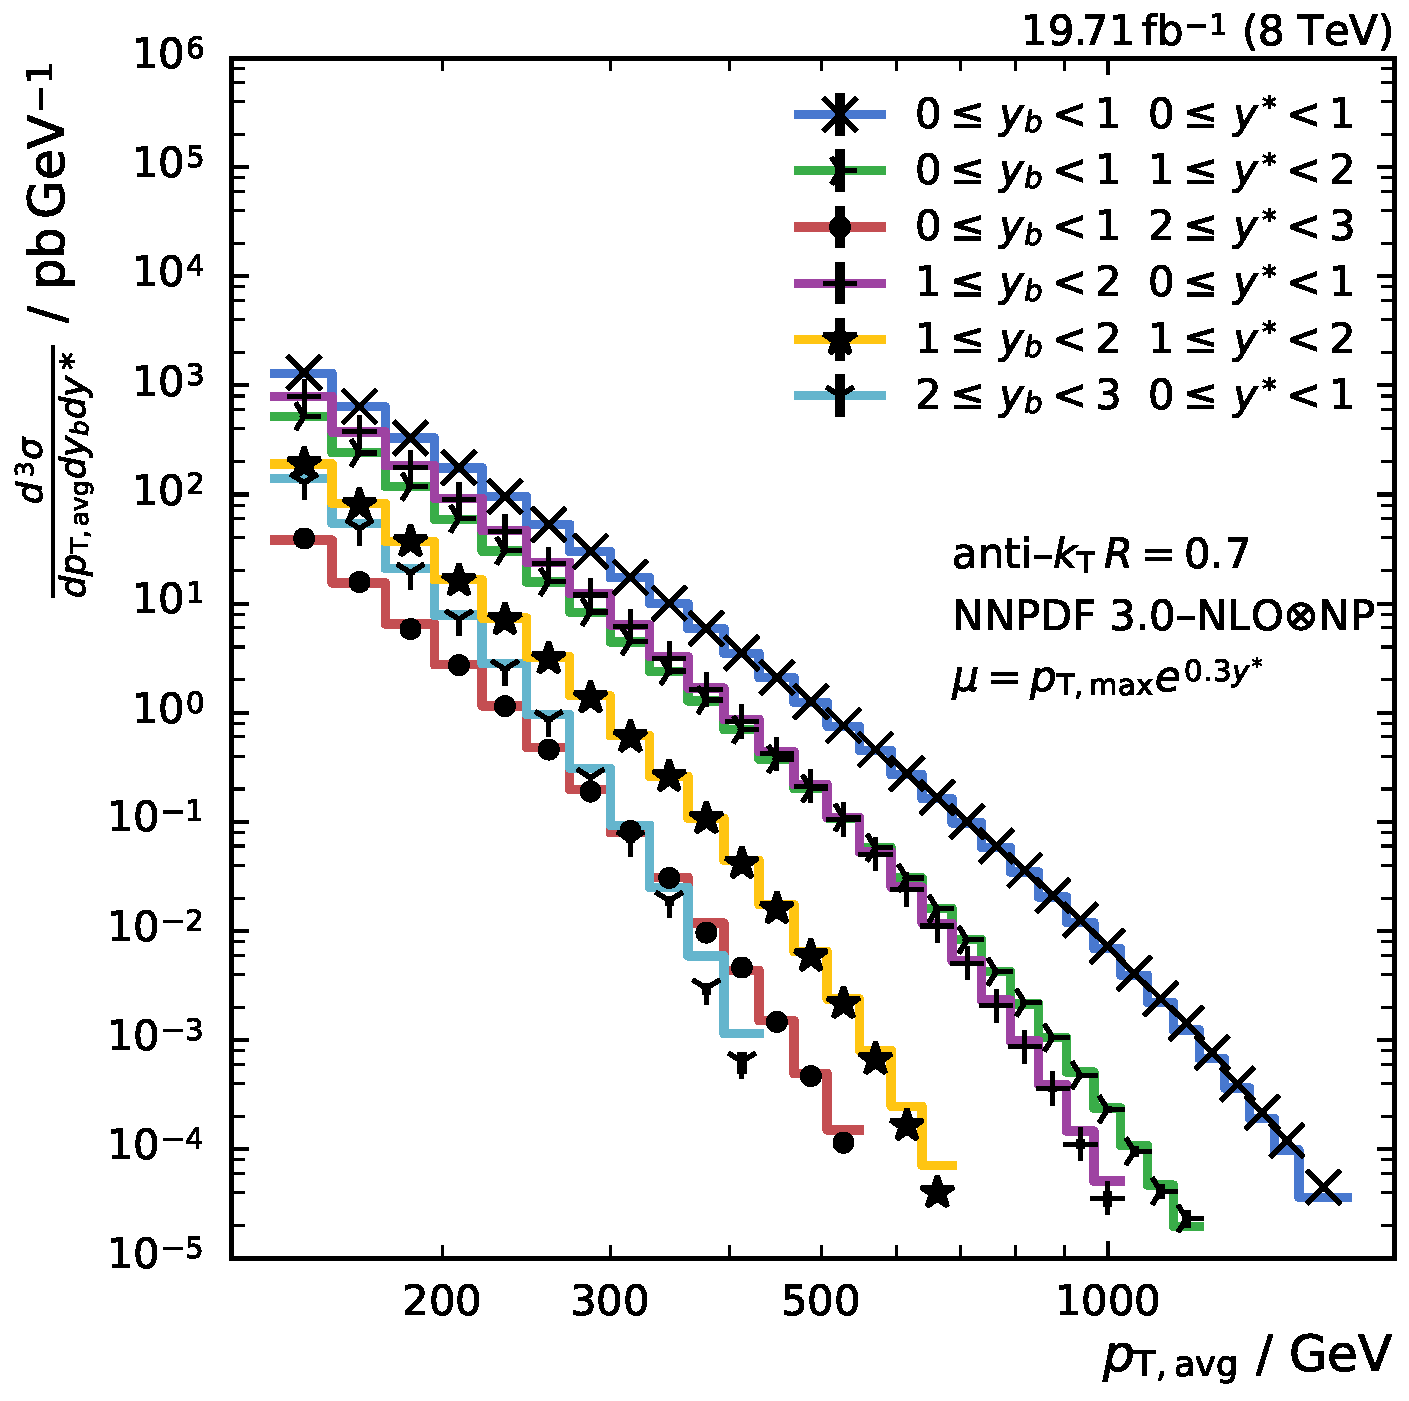
\includegraphics[width=0.47\textwidth]{figures/measurement/ptavg_spectrum.pdf}\hfill
    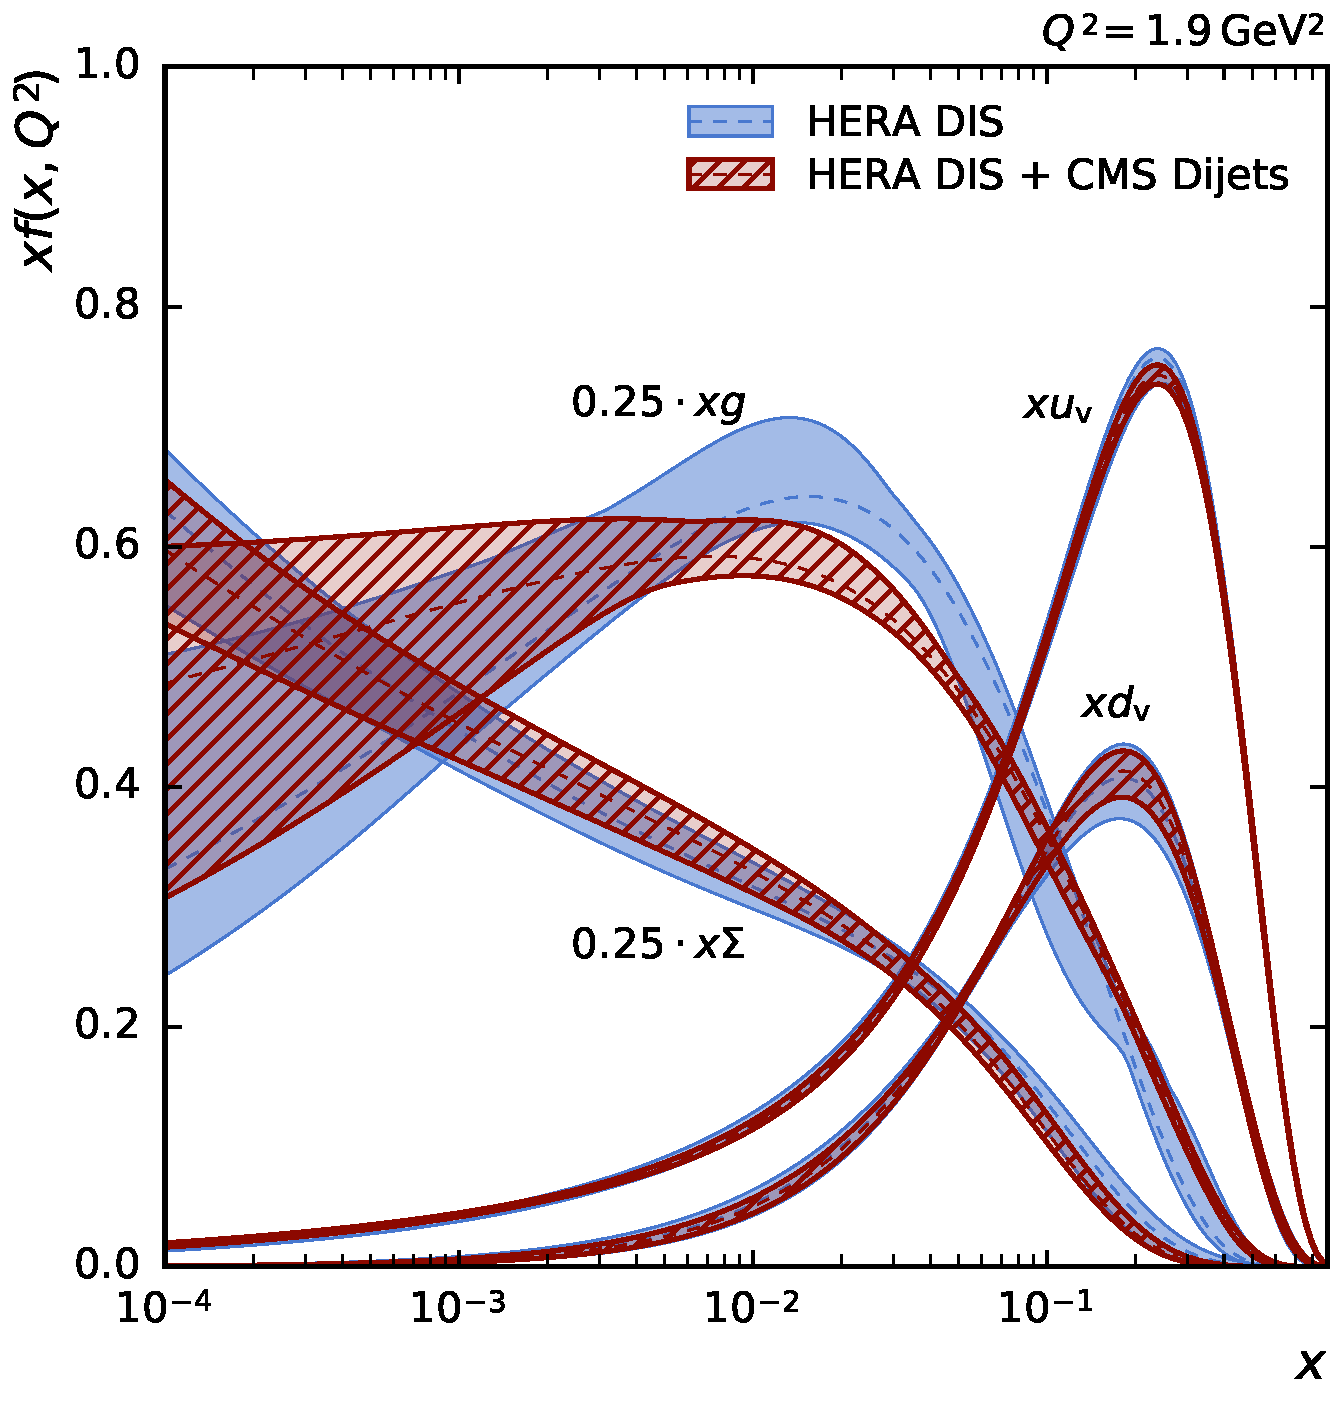
\includegraphics[width=0.45\textwidth]{figures/pdf_constraints/pdfcomp_direct_overview_1.9.pdf}
    \caption[Summary plot of results]{Left:
    The triple-differential dijet cross sections. The data are indicated by black
    markers, the NLO theory prediction by colored lines. Right: Overview of
    fitted PDFs with and without including the triple-differential dijet
    measurement.}
    \label{fig:conclusion}
\end{figure}

The measurement has been performed using the CMS detector at a center-of-mass
energy of \SI{8}{\TeV} using the complete data set recorded in 2012. A multitude
of studies of trigger, reconstruction and detector efficiencies prove the
robustness of the analysis. The measured cross sections have been corrected for
detector effects in an iterative unfolding procedure. Fig.~\ref{fig:conclusion}
left shows the cross sections in the six studied \ystar and \yboost bins.

Theoretical predictions were calculated in pQCD at NLO accuracy and were
complemented with non-perturbative corrections. The data is well
described by the theory over many orders of magnitude. In phase space regions
containing highly boosted dijet events, the data discriminate between the
predictions using different global PDF sets because of the high experimental
precision.

As a consequence, constraints on the PDFs can be provided. The sensitivity of
the PDFs is demonstrated by performing a PDF fit to DIS cross sections of the
HERA experiments and the dijet cross sections measured in this thesis. It was
found that the PDFs are improved if the dijet data are included and the
uncertainties of the PDFs, especially those of the gluon PDF, are
significantly reduced. Fig.~\ref{fig:conclusion} right demonstrates the PDF
constraints.

The strong coupling constant \asmz was determined by performing a simultaneous
fit of the PDFs and the strong coupling. The obtained value reads
%
\begin{equation*}
  \asmz = 0.1194_{-0.0015}^{+0.0015}(\mathrm{exp})_{-0.0002}^{+0.0002}(\mathrm{mod})_{-0.0004}^{+0.0002}(\mathrm{par})_{-0.0019}^{+0.0031}(\mathrm{scale})
\end{equation*}
%
and is in agreement with the world average value of $\asmz = 0.1181 \pm
0.0013$ determined by the PDG~\cite{Agashe:2014kda}. The dominant uncertainty is
of theoretical origin.

The pioneering studies presented in this thesis prove that the triple-differential
measurement of dijet cross sections using the chosen observables are an
excellent approach to perform QCD precision studies.

Two areas provide the opportunity for further improvements: In the near future,
NNLO corrections for dijet calculations will be available. The accuracy of the
cross section predictions will be improved. Especially the determination of
\asmz will profit from reduced scale uncertainties. 

The restart of the LHC at $\sqrt{s}=\SI{13}{\TeV}$ opens up a larger accessible
phase space. When CMS has collected a sufficiently large data sample, it will be
possible to extend this measurement to additional phase space regions and
improve the statistical precision.

\todo{Concluding sentence}
